\documentclass[a4paper,11pt]{report}

\usepackage{keyval}
\usepackage[utf8]{inputenc}
\usepackage[italian]{babel}
\usepackage{graphicx}
\usepackage{geometry}
\usepackage{xcolor}
\usepackage[hidelinks, pdfhighlight = /N]{hyperref}
\usepackage{bookmark}
\usepackage{longtable}
\usepackage{listingsutf8}
\usepackage{color}
\usepackage{hyperref}
\usepackage{pdfpages}
\definecolor{dkgreen}{rgb}{0,0.6,0}
\definecolor{gray}{rgb}{0.5,0.5,0.5}
\definecolor{mauve}{rgb}{0.58,0,0.82}
\lstset{language=SQL,
  inputencoding=utf8,
  literate = {à}{{\`a}}2 {À}{{\`A}}1 
  			 {ò}{{\`o}}2 {Ò}{{\`O}}1 
			 {è}{{\`e}}2 {È}{{\`E}}1 
			 {ù}{{\`u}}2 {Ù}{{\`U}}1,
  extendedchars=true,
  basicstyle={\normalsize\ttfamily},
  belowskip=3mm,
  breaklines=true,
  classoffset=0,
  columns=flexible,
  commentstyle=\color{dkgreen},
  framexleftmargin=0em,
  frameshape={}{yy}{}{}, %To remove to vertical lines on left, set frameshape={}{}{}{}
  keywordstyle=\color{blue},
  numbers=left, %If you want line numbers, set numbers=left
  numberstyle=\normalsize\color{gray},
  showstringspaces=false,
  stringstyle=\color{mauve},
  tabsize=3,
  xleftmargin =5pt,
}

\begin{document}
	\begin{titlepage}

		\newgeometry{margin = 0.4in}
		\center

		\textsc{
			\LARGE
			Università degli studi di napoli federico II\\
			Scuola Politecnica e delle Scienze di Base\\
			\Large
			Dipartimento di Ingegneria Elettrica e Tecnologie dell'Informazione\\
		}

		
\includegraphics[width = 140pt]{IMGs/Logo_unina.png}

		\textsc{
			\normalsize
			CORSO DI LAUREA IN INFORMATICA\\
			INSEGNAMENTO DI OBJECT ORIENTATION\\
			ANNO ACCADEMICO 2020/2021\\			
		}

		\vspace{4cm}

		\Huge
		\textbf{
			Progettazione e sviluppo di un applicativo in Java per un\\
			SISTEMA DI PLANNING PER GESTIONE DI PROGETTI
		}
		
		\vspace{6cm}


		\begin{minipage}[t]{0.4\textwidth}

			\begin{flushleft}

				\Large
				\textbf{Autori:}\\
				~\\
				\large
				Bianca Giada CHEHADE\\
				MATRICOLA N86003209\\
				b.chehade@studenti.unina.it\\
				~\\
				Francesco Rosario ZAZA\\
				MATRICOLA N86002501\\
				fra.zaza@studenti.unina.it\\

			\end{flushleft}

		\end{minipage}
		~
		\begin{minipage}[t]{0.4\textwidth}

			\begin{flushright}

				\Large
				\textbf{Professori}\\
				~\\
				\large
				Prof. Sergio DI MARTINO\\

			\end{flushright}

		\end{minipage}
		
		\author{}
		\date{}

	\end{titlepage}
	\part*{Questa pagina è stata lasciata intenzionalmente bianca.}
	\newgeometry{tmargin = 0.2in, bmargin = 0.8in}
	\tableofcontents
	\newgeometry{tmargin = 1.5cm, bmargin = 0.8in}
	\chapter{Descrizione del progetto}
		\section{Traccia del progetto}
			Si sviluppi un sistema informativo, composto da una base di dati relazionale e un applicativo Java dotato di
			GUI (Swing o JavaFX), per la gestione di progetti in un’azienda. Si tenga traccia dei partecipanti al progetto,
			identificando i ruoli per ognuno di essi (per ogni progetto ci sarà solo un project manager).\\ 
			Ad ogni progetto è associata una tipologia (“Ricerca di base”, “Ricerca Industriale”, “Ricerca sperimentale”, “Sviluppo
			Sperimentale”, ...) ed uno o più ambiti (Economia, Medicina, ...). Il sistema dovrà permettere anche
			l'organizzazione di meeting fisicamente, in sale riunioni, o telematicamente su una piattaforma di
			videoconferenza. Si dovrà tenere traccia delle partecipazioni ai progetti ed ai meeting, ai fini della valutazione
			del singolo partecipante. In fase di creazione di un nuovo progetto, i partecipanti dovranno essere selezionati
			in base a criteri di ricerca che includono anche il salario medio e la valutazione aziendale del partecipante,
			oltre alla tipologia di progetti cui ha preso parte.
		
		\section{Descrizione sintetica}
			Si progetterà ed implementerà un applicativo in Java  
			per un sistema di planning di progetti chiamato \textbf{Projesting}.\\
			Una volta effettuato l'accesso tramite Partita IVA, sarà possibile per l'azienda:
			\begin{itemize} 
				\item Creare un nuovo progetto specificandone il \textit{Project Manager}, la tipologia, gli ambiti e il budget concordato con il commissionante, che 
				può essere una società o un cliente privato;
				\item Visualizzare tutti i progetti attualmente attivi;
				\item Aggiornare il salario di un dipendente.
			\end{itemize}
			Effettuando, invece, l'accesso come dipendente dell'azienda, sarà possibile usufruire di diverse funzionalità
			a seconda del proprio ruolo: \textit{Project Manager} o progettista qualsiasi.
			Per il \textit{Project Manager}, sarà possibile:
			\begin{itemize}
				\item Creare un team di lavoro specificando un ruolo per ciascun progettista;
				\item Visualizzare informazioni sui dipendenti liberi;
				\item Visualizzare informazioni sui singoli progettisti e sui loro progetti passati;
				\item Programmare un meeting;
				\item Aggiornare lo stato di un meeting;
				\item Chiudere il progetto ed inserire le valutazioni per i progettisti.
			\end{itemize} 
			\newpage
			Per i progettisti, sarà possibile:
			\begin{itemize}
				\item Visualizzare i meeting a cui si è iscritti;
				\item Iscriversi ad un meeting;
				\item Visualizzare le informazioni sul progetto.
			\end {itemize}
	\chapter{Progettazione}
		\section{Class Diagram del progetto}
		Di seguito il Class Diagram che descrive l'applicativo, comprendente le classi
		e le relazioni che intercorrono tra esse.\\\\\\
			\includegraphics[width = \textwidth]{IMGs/Class Diagram1.pdf}
		\newpage
		\section{Sequence Diagrams}
			Di seguito i Sequence Diagrams che forniscono un esempio del workflow del codice durante l'esecuzione.
			\subsection{Controller: insertProjectTopics}
				Questo metodo è contenuto nel \texttt{Controller}, e serve ad inserire uno o più ambiti per un progetto.\\\\\\
				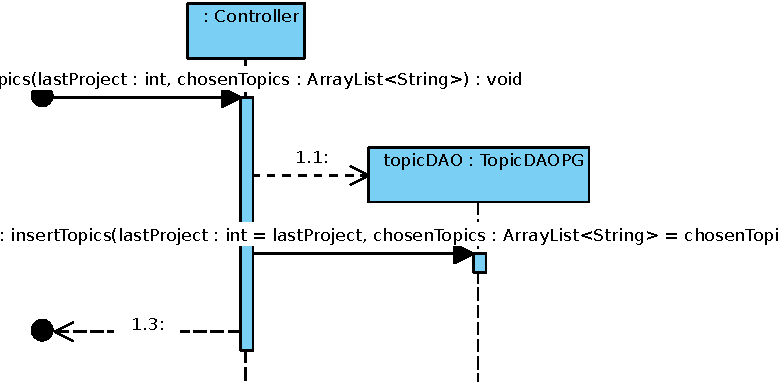
\includegraphics[width = \textwidth]{IMGs/insertProjectTopicsDiagram.pdf}
			\subsection{Controller: fillEmployeeForLogin}
				Questo metodo è contenuto nel \texttt{Controller}, e permette di recuperare tutte le informazioni relative 
				a un dipendente appena dopo il login.\\\\\\
			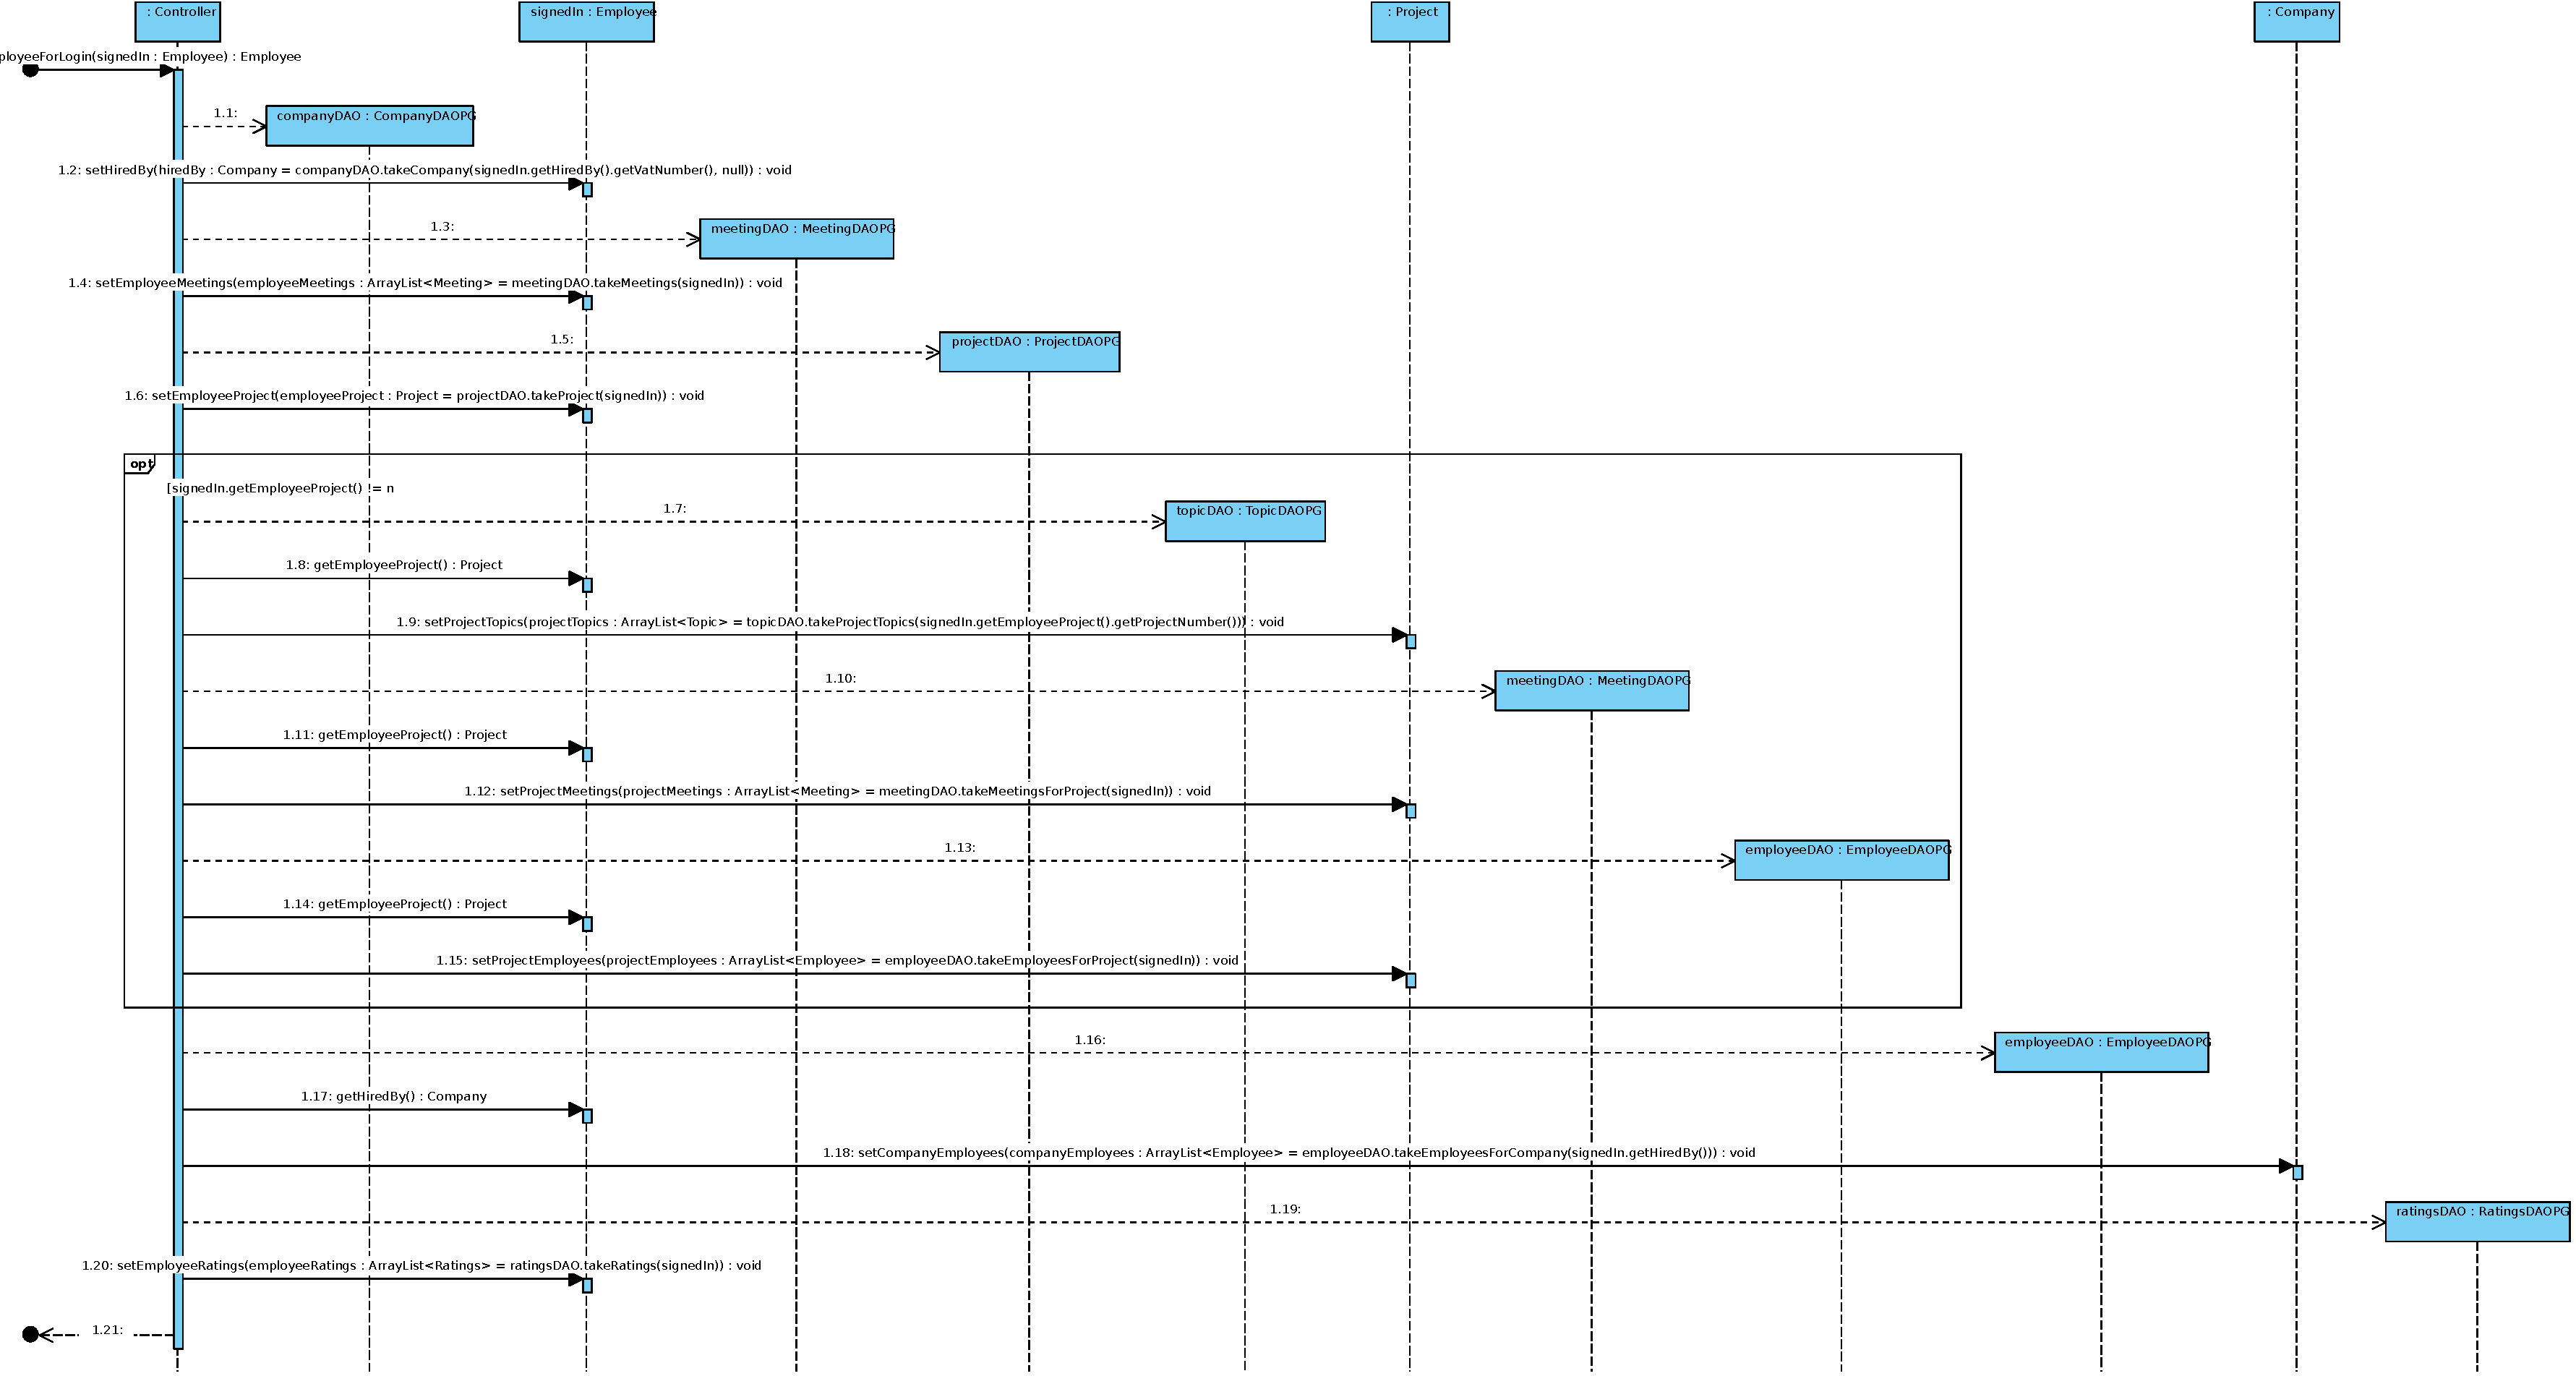
\includegraphics[width = \textwidth]{IMGs/fillEmployeeDiagram.pdf}
		\newpage
		\section{CRC Cards}
			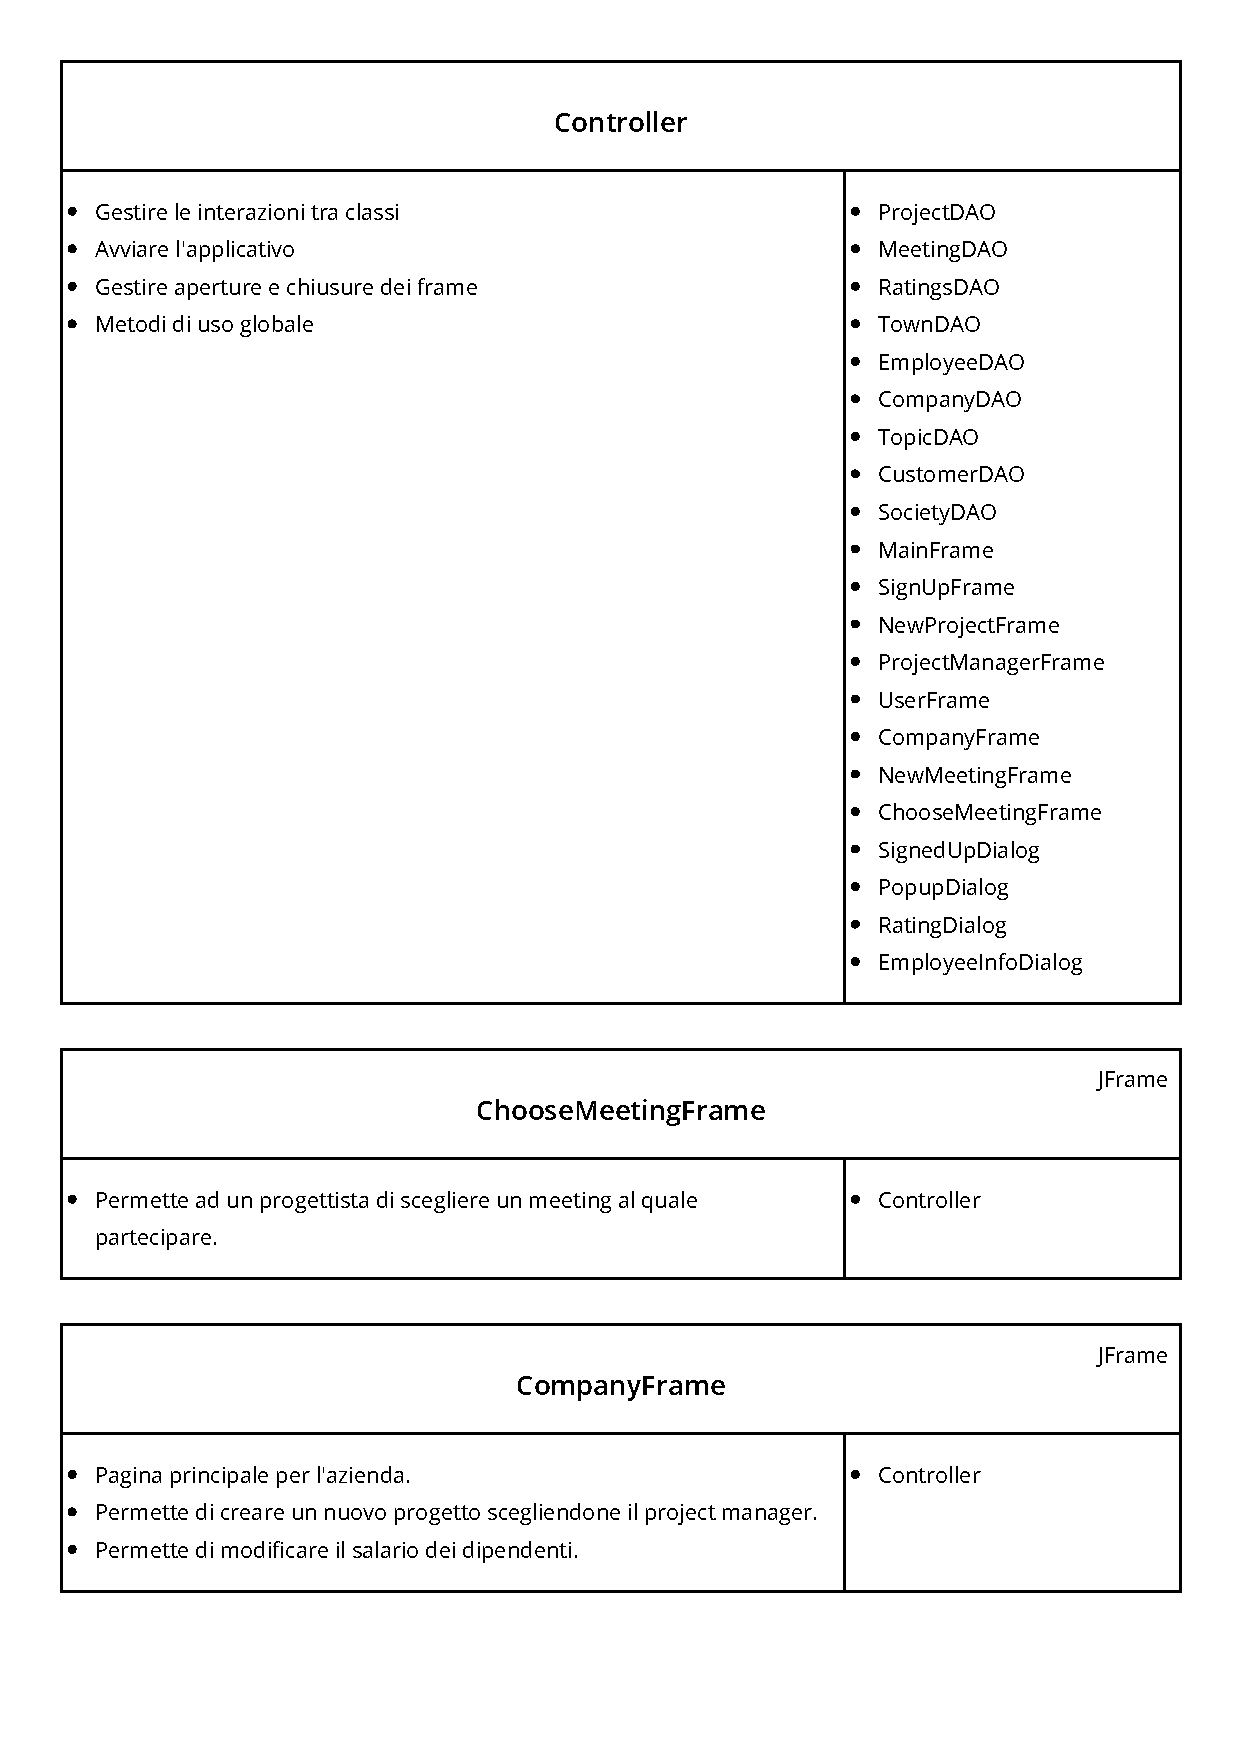
\includegraphics[page = 1, width = \textwidth]{IMGs/CRC.pdf}
			\newpage
			\includegraphics[page = 2, width = \textwidth]{IMGs/CRC.pdf}
			\newpage
			\includegraphics[page = 3, width = \textwidth]{IMGs/CRC.pdf}
			\newpage
			\includegraphics[page = 4, width = \textwidth]{IMGs/CRC.pdf}
			\newpage
			\includegraphics[page = 5, width = \textwidth]{IMGs/CRC.pdf}
			\newpage
			\includegraphics[page = 6, width = \textwidth]{IMGs/CRC.pdf}
\end{document}